\chapter{DUNE Physics}
\label{ch:exec-summ-physics}

DUNE will address fundamental questions key to our understanding of the universe. These include:
\begin{itemize}
   \item {\bf What is the origin of the matter-antimatter asymmetry in the universe?}
      Immediately after the Big Bang, matter and antimatter were created equally, but 
      now matter dominates.  By studying the properties of neutrino and antineutrino oscillations, 
      LBNF/DUNE will pursue the current most promising avenue for understanding this asymmetry.
   \item {\bf What are the fundamental underlying symmetries of the universe?} 
      The patterns of mixings and masses between the particles of the Standard Model 
      is not understood. By making precise measurements of the mixing between the neutrinos 
      and the ordering of neutrino masses and comparing these with the quark sector, 
      LNBF/DUNE could reveal new underlying symmetries of the universe.
  \item{\bf  Is there a Grand Unified Theory of the Universe?} 
      Results from a range of experiments suggest that the physical forces observed today 
      were unified into one force at the birth of the universe.  Grand Unified Theories (GUTs), 
      which attempt to describe the unification of forces, predict that protons should decay, 
      a process that has never been observed. DUNE will search for proton decay in the range of 
      proton lifetimes predicted by a wide range of GUT models.
   \item{\bf How do supernovae explode and what new physics will we learn from a neutrino burst?}
      Many of the heavy elements that are the key components of life were created in the 
      super-hot cores of collapsing stars.  DUNE would be able to detect the neutrino bursts 
      from core-collapse supernovae within our galaxy (should any occur).  Measurements of the 
      time, flavor and energy structure of the neutrino burst will be critical for understanding 
      the dynamics of this important astrophysical phenomenon, as well as bringing information 
      on neutrino properties and other particle physics.
\end{itemize}

%%%%%%%%%%%%%%%%%%%%%%%%%%%%%%%%%%%%%%%%%%%%%%%%%%%%%%%%%%%%%%%%%%%%
\section{Introduction: Scientific Goals}
\label{sec:exec-summ-physics-goals}


The DUNE scientific objectives are categorized into: the \textit{primary science program}, addressing the key science questions 
highlighted by the particle physics project prioritization panel (P5); 
a high-priority \textit{ancillary science program} that is 
enabled by the construction of LBNF and DUNE; and \textit{additional scientific objectives}, that may require further developments 
of the LArTPC technology. A detailed description of the physics objectives of DUNE is provided in \href{http://arxiv.org/abs/1512.06148}{Volume 2 of the DUNE Conceptual Design Report}.

%%%%%%%%%%%%%%%%%%%%%%%%%%%%
\subsection{The Primary Science Program}

The primary science program of LBNF/DUNE  focuses on fundamental open questions in neutrino and astroparticle physics: 
\begin{itemize}
  \item precision measurements of the parameters that govern $\nu_{\mu} \rightarrow \nu_\text{e}$ and
           $\overline{\nu}_{\mu} \rightarrow \overline{\nu}_\text{e}$ oscillations with the goal of
  \subitem -- measuring the charge-parity (CP) violating phase $\delta_\text{CP}$, where a value differing from zero or $\pi$ would represent the discovery of CP violation in the leptonic sector, providing a possible explanation for the matter-antimatter asymmetry in the universe;
  \subitem -- determining the neutrino mass ordering (the sign of $\Delta m^2_{31} \equiv m_3^2-m_1^2$), often referred to as the neutrino \textit{mass hierarchy}; and
  \subitem -- precision tests of the three-flavor neutrino oscillation paradigm through studies of muon neutrino disappearance 
    and electron neutrino appearance in both $\nu_\mu$ and $\overline{\nu}_{\mu}$ beams, including the 
    measurement of the mixing angle $\theta_{23}$ and the determination of the octant in which this angle lies.
    \item search for proton decay in several important decay modes, for example $\text{p}\rightarrow\text{K}^+\overline{\nu}$, where the observation of proton decay would represent a ground-breaking discovery in physics, providing a portal to Grand Unification of the forces; and
    \item detection and measurement of the $\nu_\text{e}$ flux from a core-collapse supernova within our galaxy, should one occur during the lifetime of the DUNE experiment.
\end{itemize}

%%%%%%%%%%%%%%%%%%%%%%%%%%%%%
\subsection{The Ancillary Science Program}

The intense neutrino beam from LBNF, the massive DUNE LArTPC far detector and the high-resolution
  DUNE near detector provide a rich ancillary science program, beyond the primary mission of the experiment. The ancillary science program includes
\begin{itemize}
     \item other accelerator-based neutrino flavor transition measurements with sensitivity to Beyond Standard Model (BSM) physics, such as: non-standard interactions (NSIs); the search for sterile neutrinos at both the near and far sites;
 and measurements of tau neutrino appearance;
     \item measurements of neutrino oscillation phenomena using atmospheric neutrinos;
     \item a rich neutrino interaction physics program utilizing the DUNE near detector, including: a wide-range of measurements of neutrino cross sections; studies of nuclear effects, including neutrino final-state interactions; measurements of the structure of nucleons; and  measurement of $\sin^2\theta_\text{W}$; and
     \item  the search for signatures of dark matter.
\end{itemize} 

Furthermore, a number of previous breakthroughs in particle physics have been serendipitous, in the sense that they were beyond the
original scientific objectives of an experiment. The intense LBNF neutrino beam and novel capabilities for both 
the DUNE near and far detectors will probe new regions of parameter space for both the accelerator-based and astrophysical frontiers, 
providing the opportunity for discoveries that are not currently anticipated.

\subsection{Context for Discussion of Science Capabilities in this Document}

The sections that follow highlight the projected capabilities of DUNE to realize the science program 
summarized above. These are documented in detail in \href{http://arxiv.org/abs/1512.06148}{Volume 2 
of the DUNE Conceptual Design Report}.  Since publication of the CDR in late 2015, the DUNE science 
collaboration has undertaken a campaign to develop data analysis tools and strategies in order to aid 
in detector design optimization as well as to obtain a more rigorous understanding of experimental 
sensitivity.  This campaign is in progress as of this writing, and the outcomes will be reported 
as a component of the DUNE Technical Design Report now in development.  Additionally, with 
currently-operating experiments beginning to reach peak fractional rates of integrated exposure, 
the rapid evolution of the world-wide experimental landscape in neutrino physics is particularly acute 
at present.  Thus, for the purposes of the present report, the discussion of capabilities here 
will reflect what is documented within the CDR unless otherwise noted.

%%%%%%%%%%%%%%%%%%%%%%%%%%%%%%%%%%%%%%%%%%%%%%%%%%%%%%%%%%%%%%%%%%%%
\section{Long-Baseline Neutrino Oscillation physics program}
\label{sec:exec-summ-physics-osc}

%\fixme{6 pages}
Precision neutrino oscillation measurements lie at the heart of the DUNE scientific program.
The \SIadj{1300}{\km} baseline, coupled with the wide-band
high-intensity neutrino beam from LBNF, establishes one of DUNE's key
strengths, namely sensitivity to the matter effect. This effect leads to a
discrete asymmetry in the \numu $\to$ \nue versus \anumu $\to$ \anue
oscillation probabilities, the sign of which depends on the presently
unknown mass hierarchy (MH).  At \SI{1300}{\km} the asymmetry,
\begin{equation}
\mathcal{A} = \frac{ P(\nu_\mu \rightarrow \nu_e)-P(\bar{\nu}_\mu \rightarrow \bar{\nu}_e)}{P(\nu_\mu \rightarrow \nu_e)+P(\bar{\nu}_\mu \rightarrow \bar{\nu}_e)}
\end{equation}
is approximately $\pm 40\%$ in the region of the peak flux in the
absence of CP-violating effects. This is larger than the maximal
possible CP-violating asymmetry associated with the CP-violating
phase, \deltacp, of the three-flavor PMNS mixing matrix in the region of
the peak flux. The CP asymmetry is larger in the energy regions below the peak
flux while the matter asymmetry is smaller. As a result, the LBNF
wide-band beam will allow unambiguous determination of both the MH and
\deltacp with high confidence \textit{within the same experiment}, i.e., DUNE.   

The DUNE far detector will be built as four \ktadj{10} modules, which will
come online sequentially over the course of several years. 
This staged program enables an early scientific output from DUNE, 
initially focused on the observation of natural
sources of neutrinos, searches for nucleon decay and 
measurements of background. 
Two years after commissioning the first two detector modules, 
the LBNF neutrino
beam at Fermilab will  
begin sending neutrinos over the \kmadj{1300}
baseline, commencing the LBL oscillation physics program with a beam power of up to \SI{1.2}\MW{}. Upgrades to increase the beam power to \SI{2.4}\MW{} are planned to be in place six years later.
The early physics program
will be statistically limited and constraints from comparison of the $\nu_\mu$
disappearance spectrum with that from $\nu_e$ appearance will partially mitigate systematic uncertainties. The Near Detector is expected to come online in a timescale similar to that of the initial beam and will provide powerful constraints on the beam flux and neutrino interaction model, providing the
necessary control of systematic uncertainties for the full exploitation of LBNF/DUNE. 

%The DUNE science reach is often presented in terms of  exposure expressed in units of \ktMWyr{}. For instance, seven years of data
%(\num{3.5} years in neutrino mode plus \num{3.5} years in antineutrino
%mode\footnote{unless otherwise stated, the results presented in the CDR assume equal running in neutrino and antineutrino mode.}) with a \ktadj{40} detector and a \MWadj{1.07} beam (based on a \GeVadj{80} primary proton beam) correspond to an
%exposure of \SI{300}~\ktMWyr. In some cases, we use a technically limited staging plan, described below, to present the expected sensitivity in calendar years.

The evolution of the projected DUNE sensitivities as a function of real time is estimated based on an assumed deployment plan
with the following assumptions:

\begin{itemize}
\item Year 1: \SI{20}\kt{} far detector fiducial mass, \MWadj{1.07} \GeVadj{80}
  proton beam with $1.47 \times 10^{21}$ protons-on-target per year 
  and initial ND constraints
%%%(assume \num{3}\% signal systematic)
\item Year 2: Addition of the third \ktadj{10} far detector module, for a total far detector fiducial mass of
  \SI{30}\kt
\item Year 4: Addition of the fourth \ktadj{10} far detector module, for a total far detector fiducial mass of
  \SI{40}\kt, and improved systematic constraints from ND analysis
%%%%  (assume \num{2}\% signal systematic)
 \item Year 7: Upgrade of beam power to \SI{2.14}{\MW} for a \SIadj{80}{\GeV}
  proton beam
\end{itemize}
The staging of the detectors and facility in the resource-loaded schedule leads to a similar
evolution of physics sensitivity as a function of time.
In addition, it was assumed that the knowledge from the near detector can be
retroactively applied to previous data sets, such that each
improvement in the knowledge of systematic uncertainties~\footnote{A
  detailed discussion of the systematic uncertainties assumed, given a
  near detector, is presented in %\volphys. 
  For studies without a near
  detector an uncertainty of 10\% is assumed on the unoscillated flux
  at the far detector based on the current performance of the NuMI
  beam simulation, with uncertainties on physics backgrounds $\geq
  10\%$ depending on the background.} is applied to the full exposure
up to that point.

%%%%%%%%%%%%%%%%%%%%%%%%%%%%%%%%%
\subsection{Mass Hierarchy and CP Violation}
\label{sec:exec-summ-physics-mh-cpv}

%\fixme{3 pages, spectra, numbers of events, sensitivities, plots}
%\fixme{this heading for TP was not in CDR; Anne placed it here 19/2/18}

The discriminating power between the two MH hypotheses is quantified
by the difference, denoted $\Delta \chi^2$, between the
$-2\log{\cal L}$ values calculated for the normal and inverted
hierarchies. As the sensitivity depends on the true value of the unknown
CP-violating phase, \deltacp, all possible values of \deltacp are
considered.  In terms of this test statistic\footnote{For the case of the MH determination, the usual
  association of this test statistic with a $\chi^2$ distribution for
  one degree of freedom is not strictly correct; additionally the assumption of a
  Gaussian probability density 
  implicit in this notation is not exact.}, the MH
sensitivity of DUNE for exposures of seven and ten years is
illustrated in Figure~\ref{fig:mhexec} for the case of normal
hierarchy and the NuFit 2016~\cite{nufit2016} best-fit value of \sinst{23} = 0.44. 
For this exposure, the DUNE determination of the MH will be definitive for
the overwhelming majority of the  \deltacp and \sinst{23} parameter space.
Even for unfavorable combinations of the parameters, a statistically
ambiguous outcome is highly unlikely.  
\begin{dunefigure}[Summary of mass hierarchy sensitivities]{mhexec}{The
    square root of the mass hierarchy discrimination metric $\Delta
    \chi^2$ is plotted as a function of the unknown value of \deltacp
    for exposures of seven and ten years  
    (left).  The minimum significance
    --- the lowest point on the curve on the left --- with which the mass
    hierarchy can be determined for all values of \deltacp and the significance for a true value of \deltacp=-$\pi$/2 as a
    function of years of running under the staging plan described in the text (right).
    The shaded regions represent the range in sensitivity corresponding to
    different true values of $\theta_{23}$.}
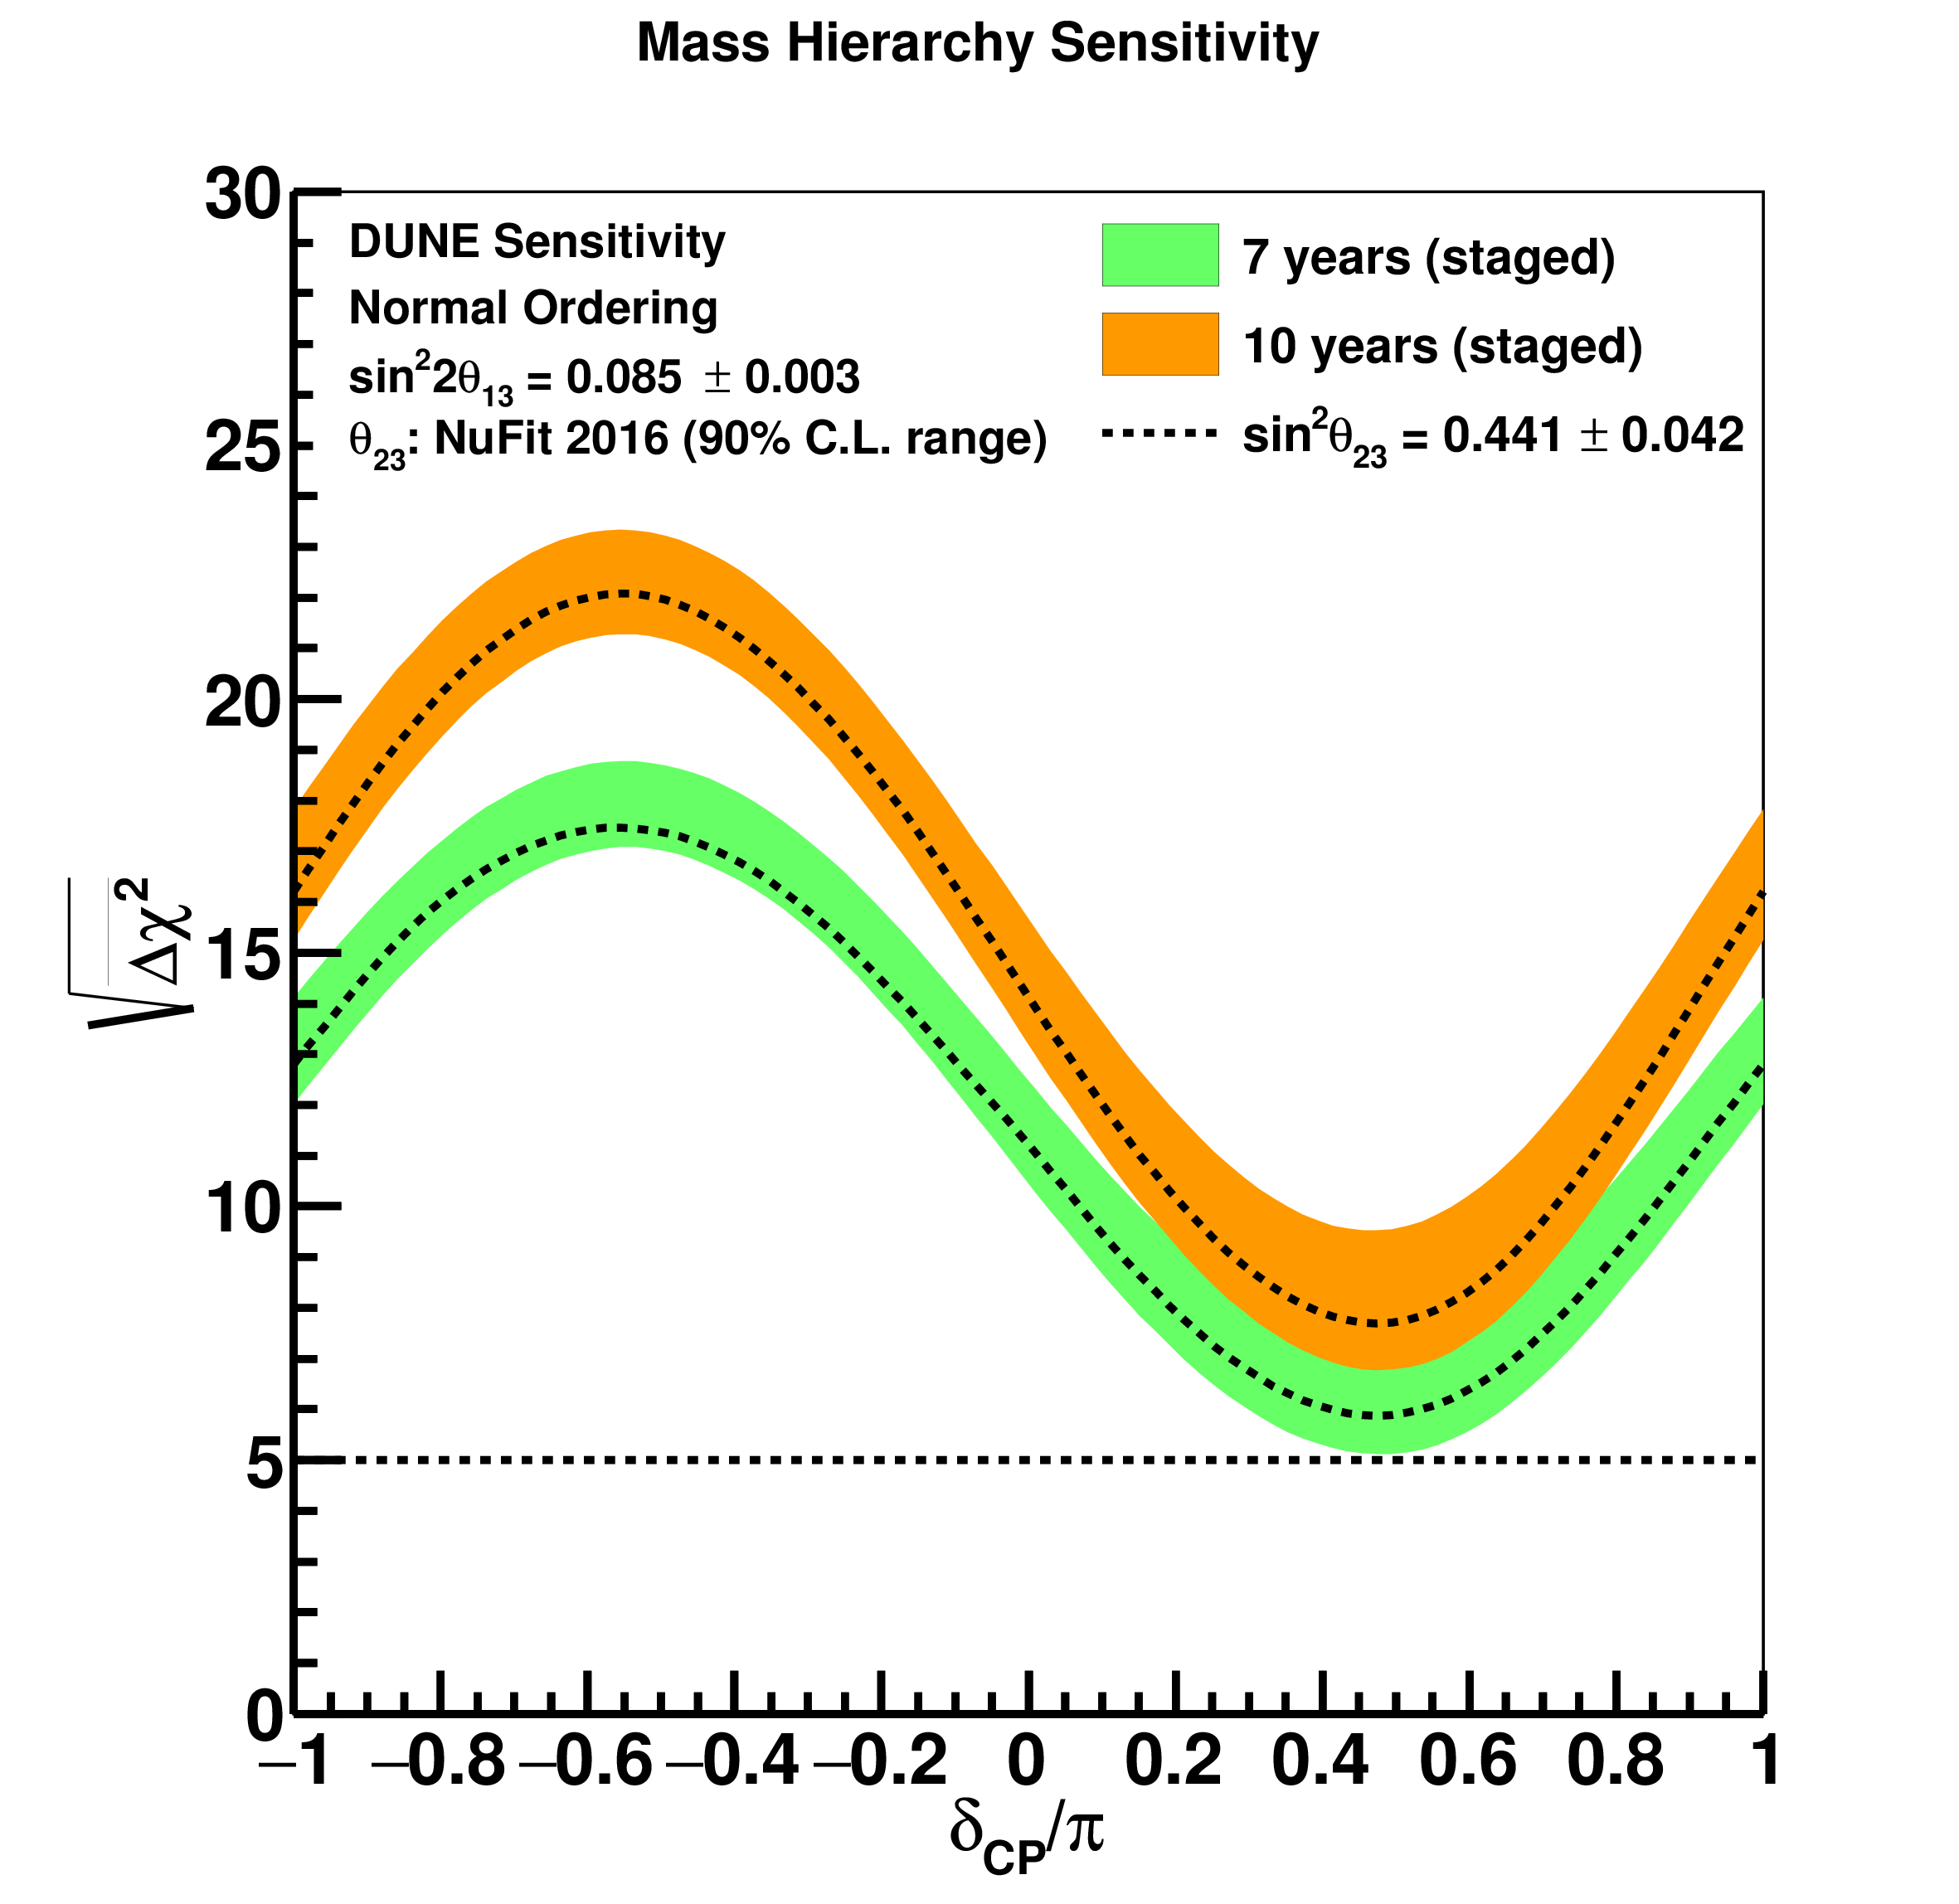
\includegraphics[width=0.49\textwidth]{mh_two_exps_th23band_no_2017.png}
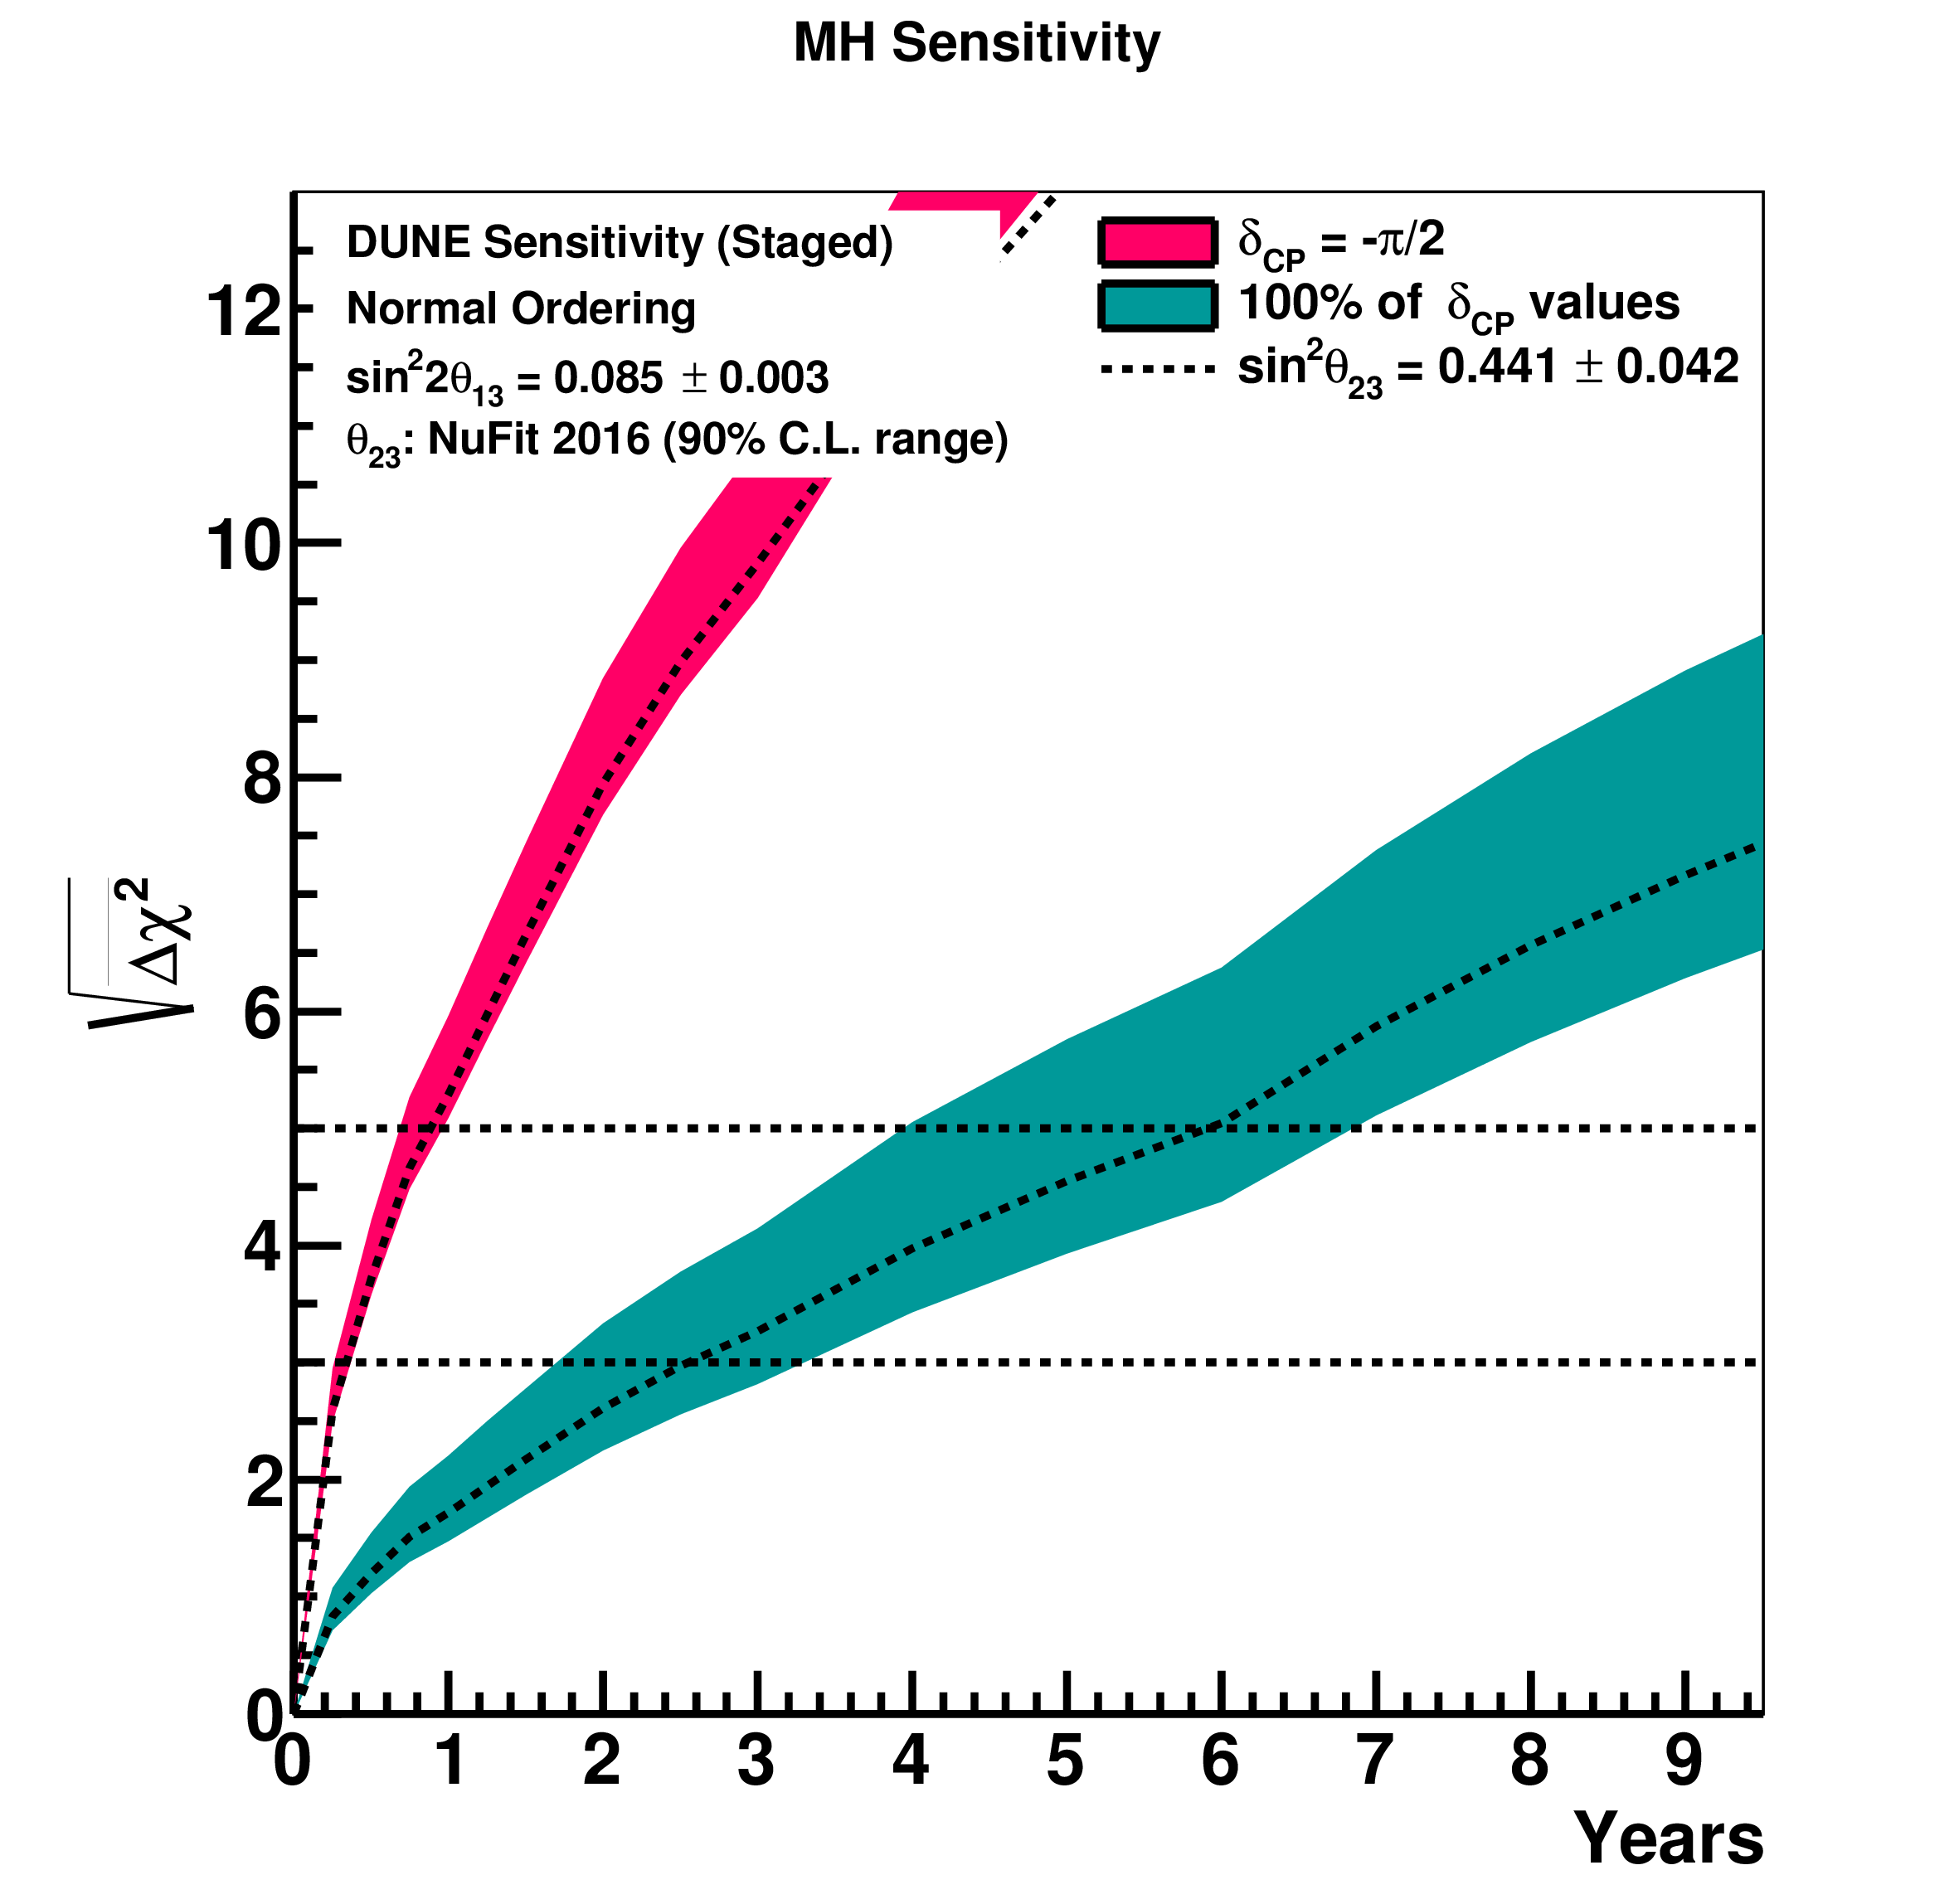
\includegraphics[width=0.49\textwidth]{mh_exp_staging_th23band_2017.png}
\label{fig:mhexec}
\end{dunefigure}


Figure~\ref{fig:mhexec} shows the evolution of the sensitivity to the MH determination as a function
of years of operation, for the least favorable scenario, corresponding to the case in which the MH asymmetry is
maximally offset by the leptonic CP asymmetry. An exposure of \SI{209}~\ktMWyr{}  
(which corresponds to approximately \num{5} years of operation) is required to distinguish
between normal and inverted hierarchy with $|\Delta \chi^2| =
\overline{|\Delta \chi^2|} = 25$.  This corresponds to a $\geq
99.9996\%$ probability of determining the correct hierarchy. 
The dependence of the mass
hierarchy sensitivity on systematics is still under evaluation, but
current studies indicate a only weak dependence on the assumptions for 
the achievable systematic uncertainties. This indicates that a measurement of the unknown
neutrino mass hierarchy with very high precision can be carried out
during the first few years of operation.
Concurrent analysis of the corresponding atmospheric-neutrino
samples in an underground detector may improve the precision and
speed with which the MH is resolved.


DUNE will search for CP violation using the \numu to \nue and \anumu
to \anue oscillation channels, with two objectives.  First, DUNE aims
to observe a signal for leptonic CP violation independent of the
underlying nature of neutrino oscillation phenomenology. Such a signal
will be observable in comparisons of $\nu_\mu \rightarrow \nu_e$ and
$\bar{\nu}_{\mu} \rightarrow \bar{\nu}_e$ oscillations of the LBNF
beam neutrinos in a wide range of neutrino energies over the
\SIadj{1300}{\km} baseline.
Second,
DUNE aims to make a precise determination of the value of \deltacp
within the context of the standard three-flavor mixing scenario
described by the PMNS neutrino mixing matrix. Together, the pursuit of
these two goals provides a thorough test of the standard three-flavor
scenario.

\begin{dunefigure}[CP-violation sensitivity and $\delta_{\rm CP}$
  resolution as a function of exposure]{execsummaryCP}{The
    significance with which CP violation can be determined for 75\% and 50\% of
    \deltacp values and for \deltacp=-$\pi$/2 (left) and the expected 1$\sigma$ resolution
    (right) as a function of exposure in years using the proposed
    staging plan outlined in this chapter. The shaded regions
    represent the range in sensitivity corresponding to
    different true values of $\theta_{23}$. The plots assume normal mass hierarchy.}
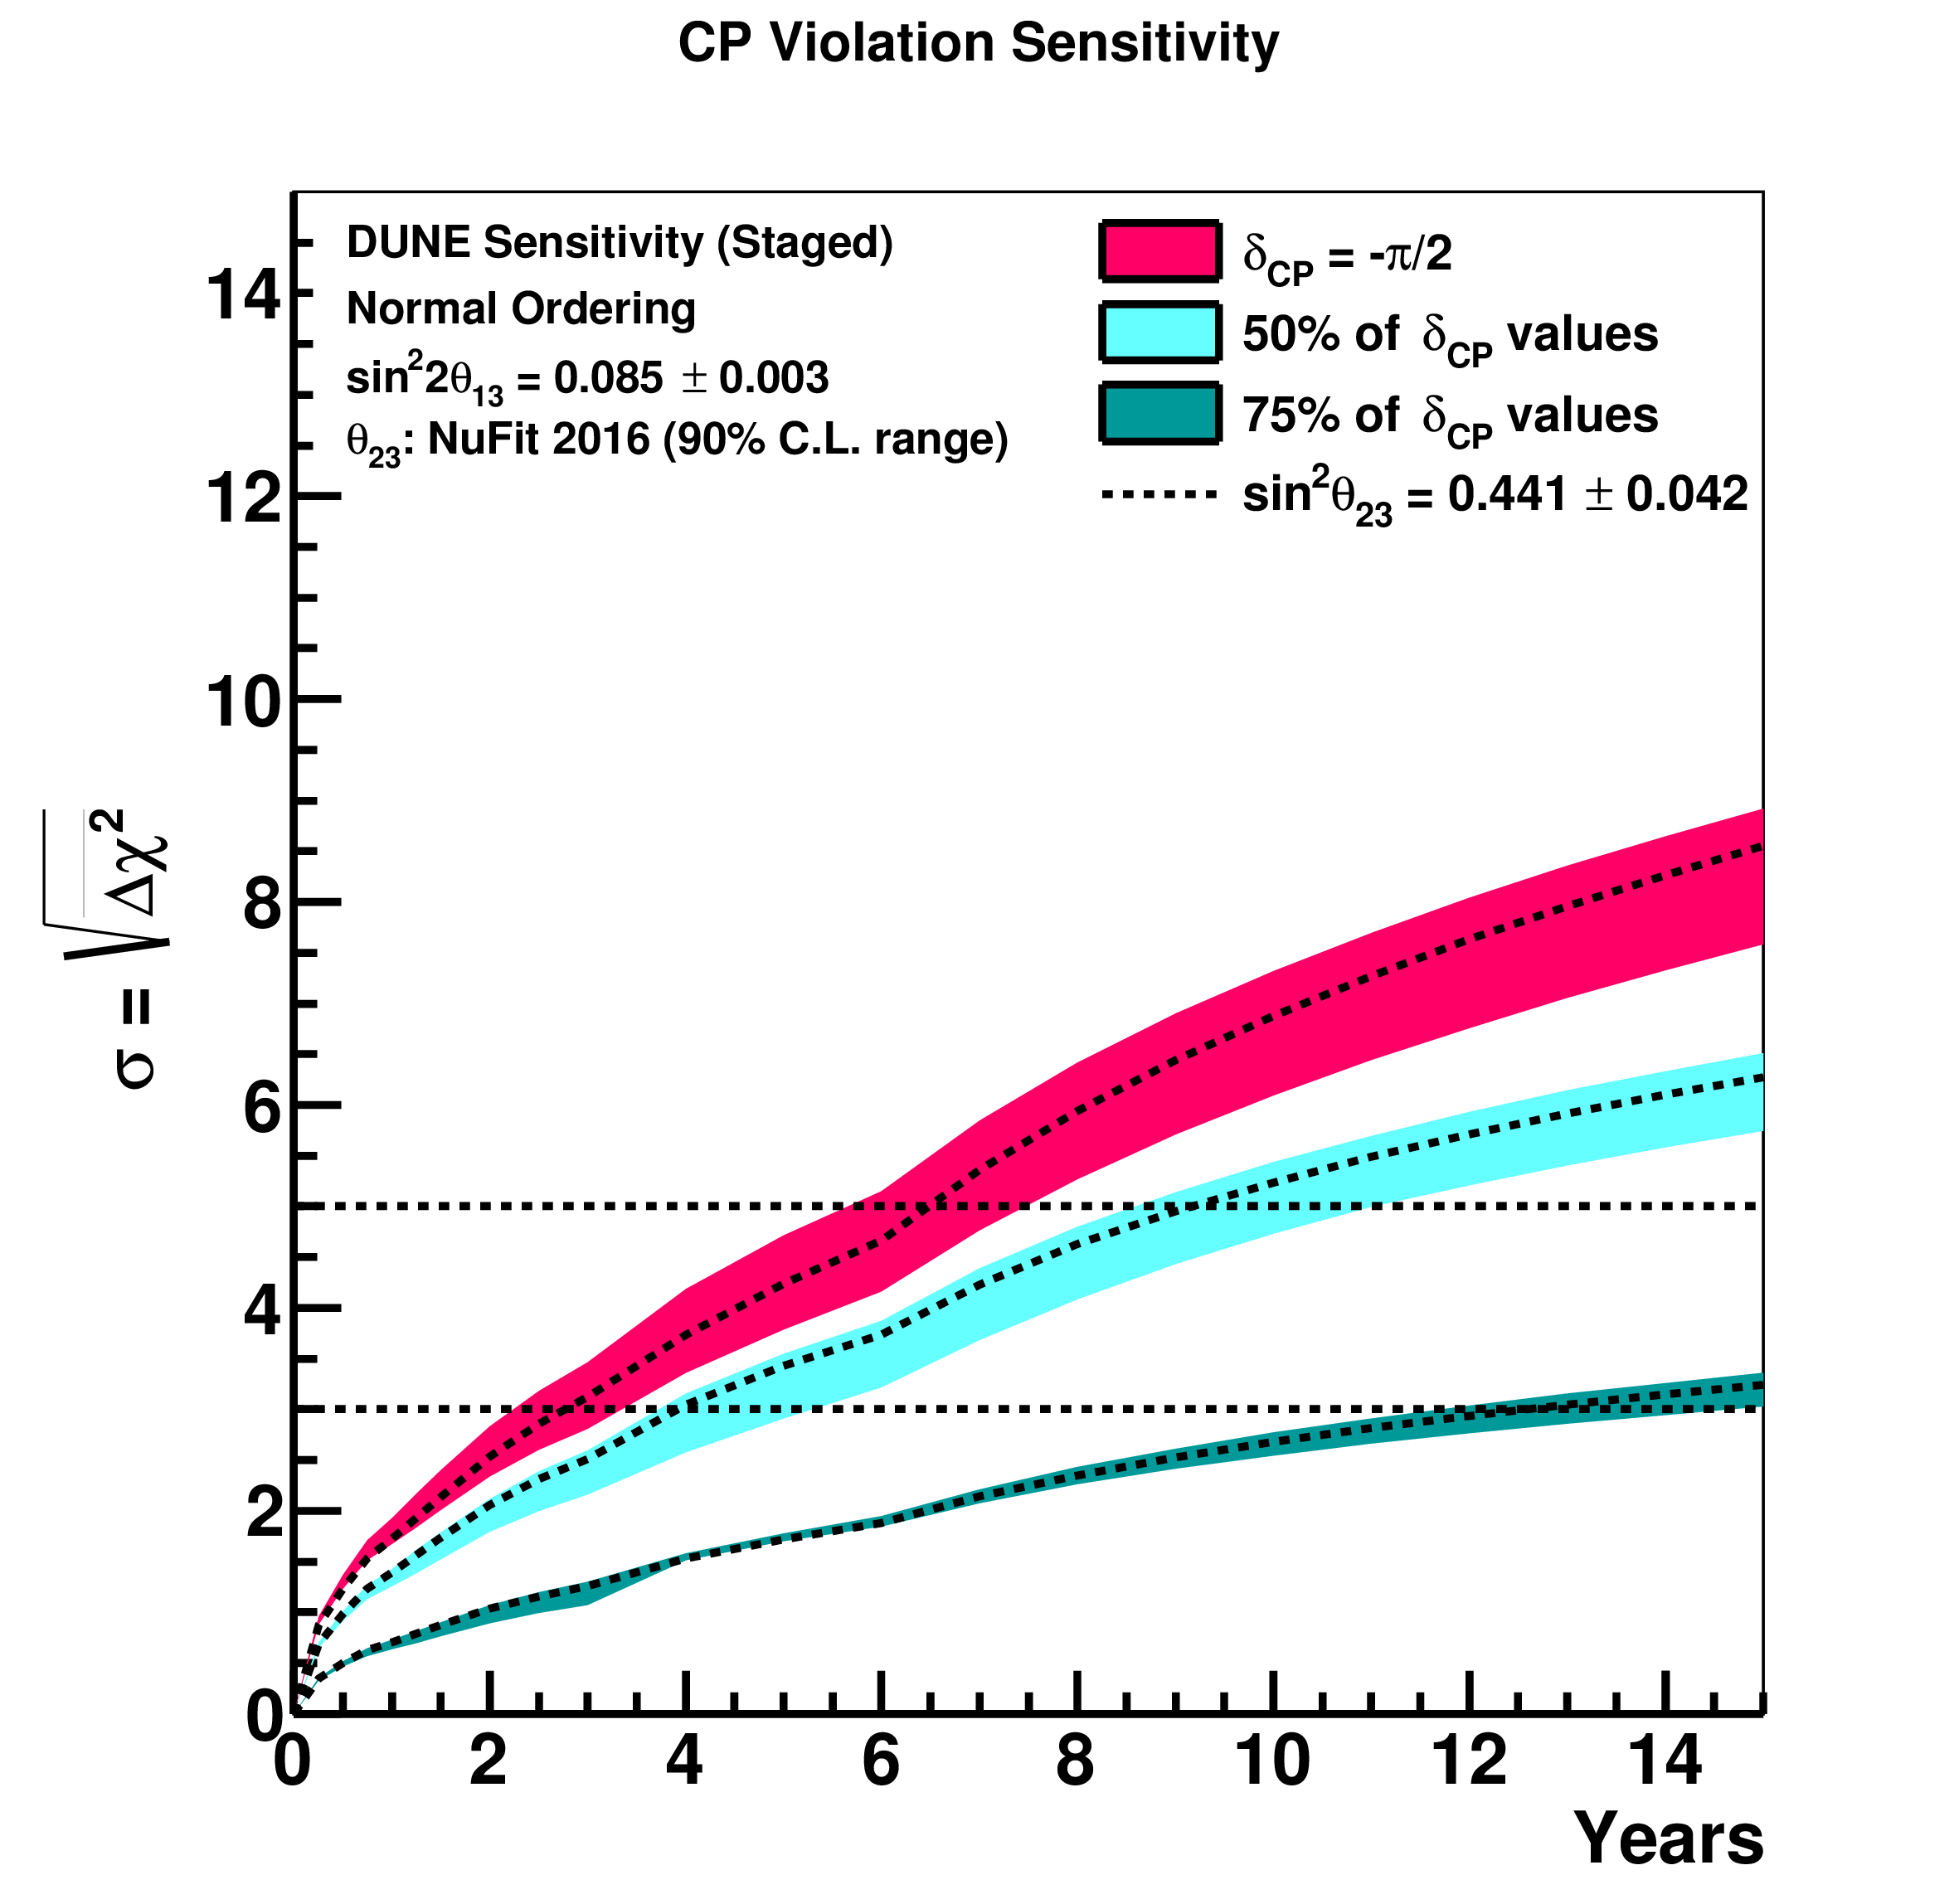
\includegraphics[width=0.49\textwidth]{cpv_exp_staging_th23band_2017.png}
 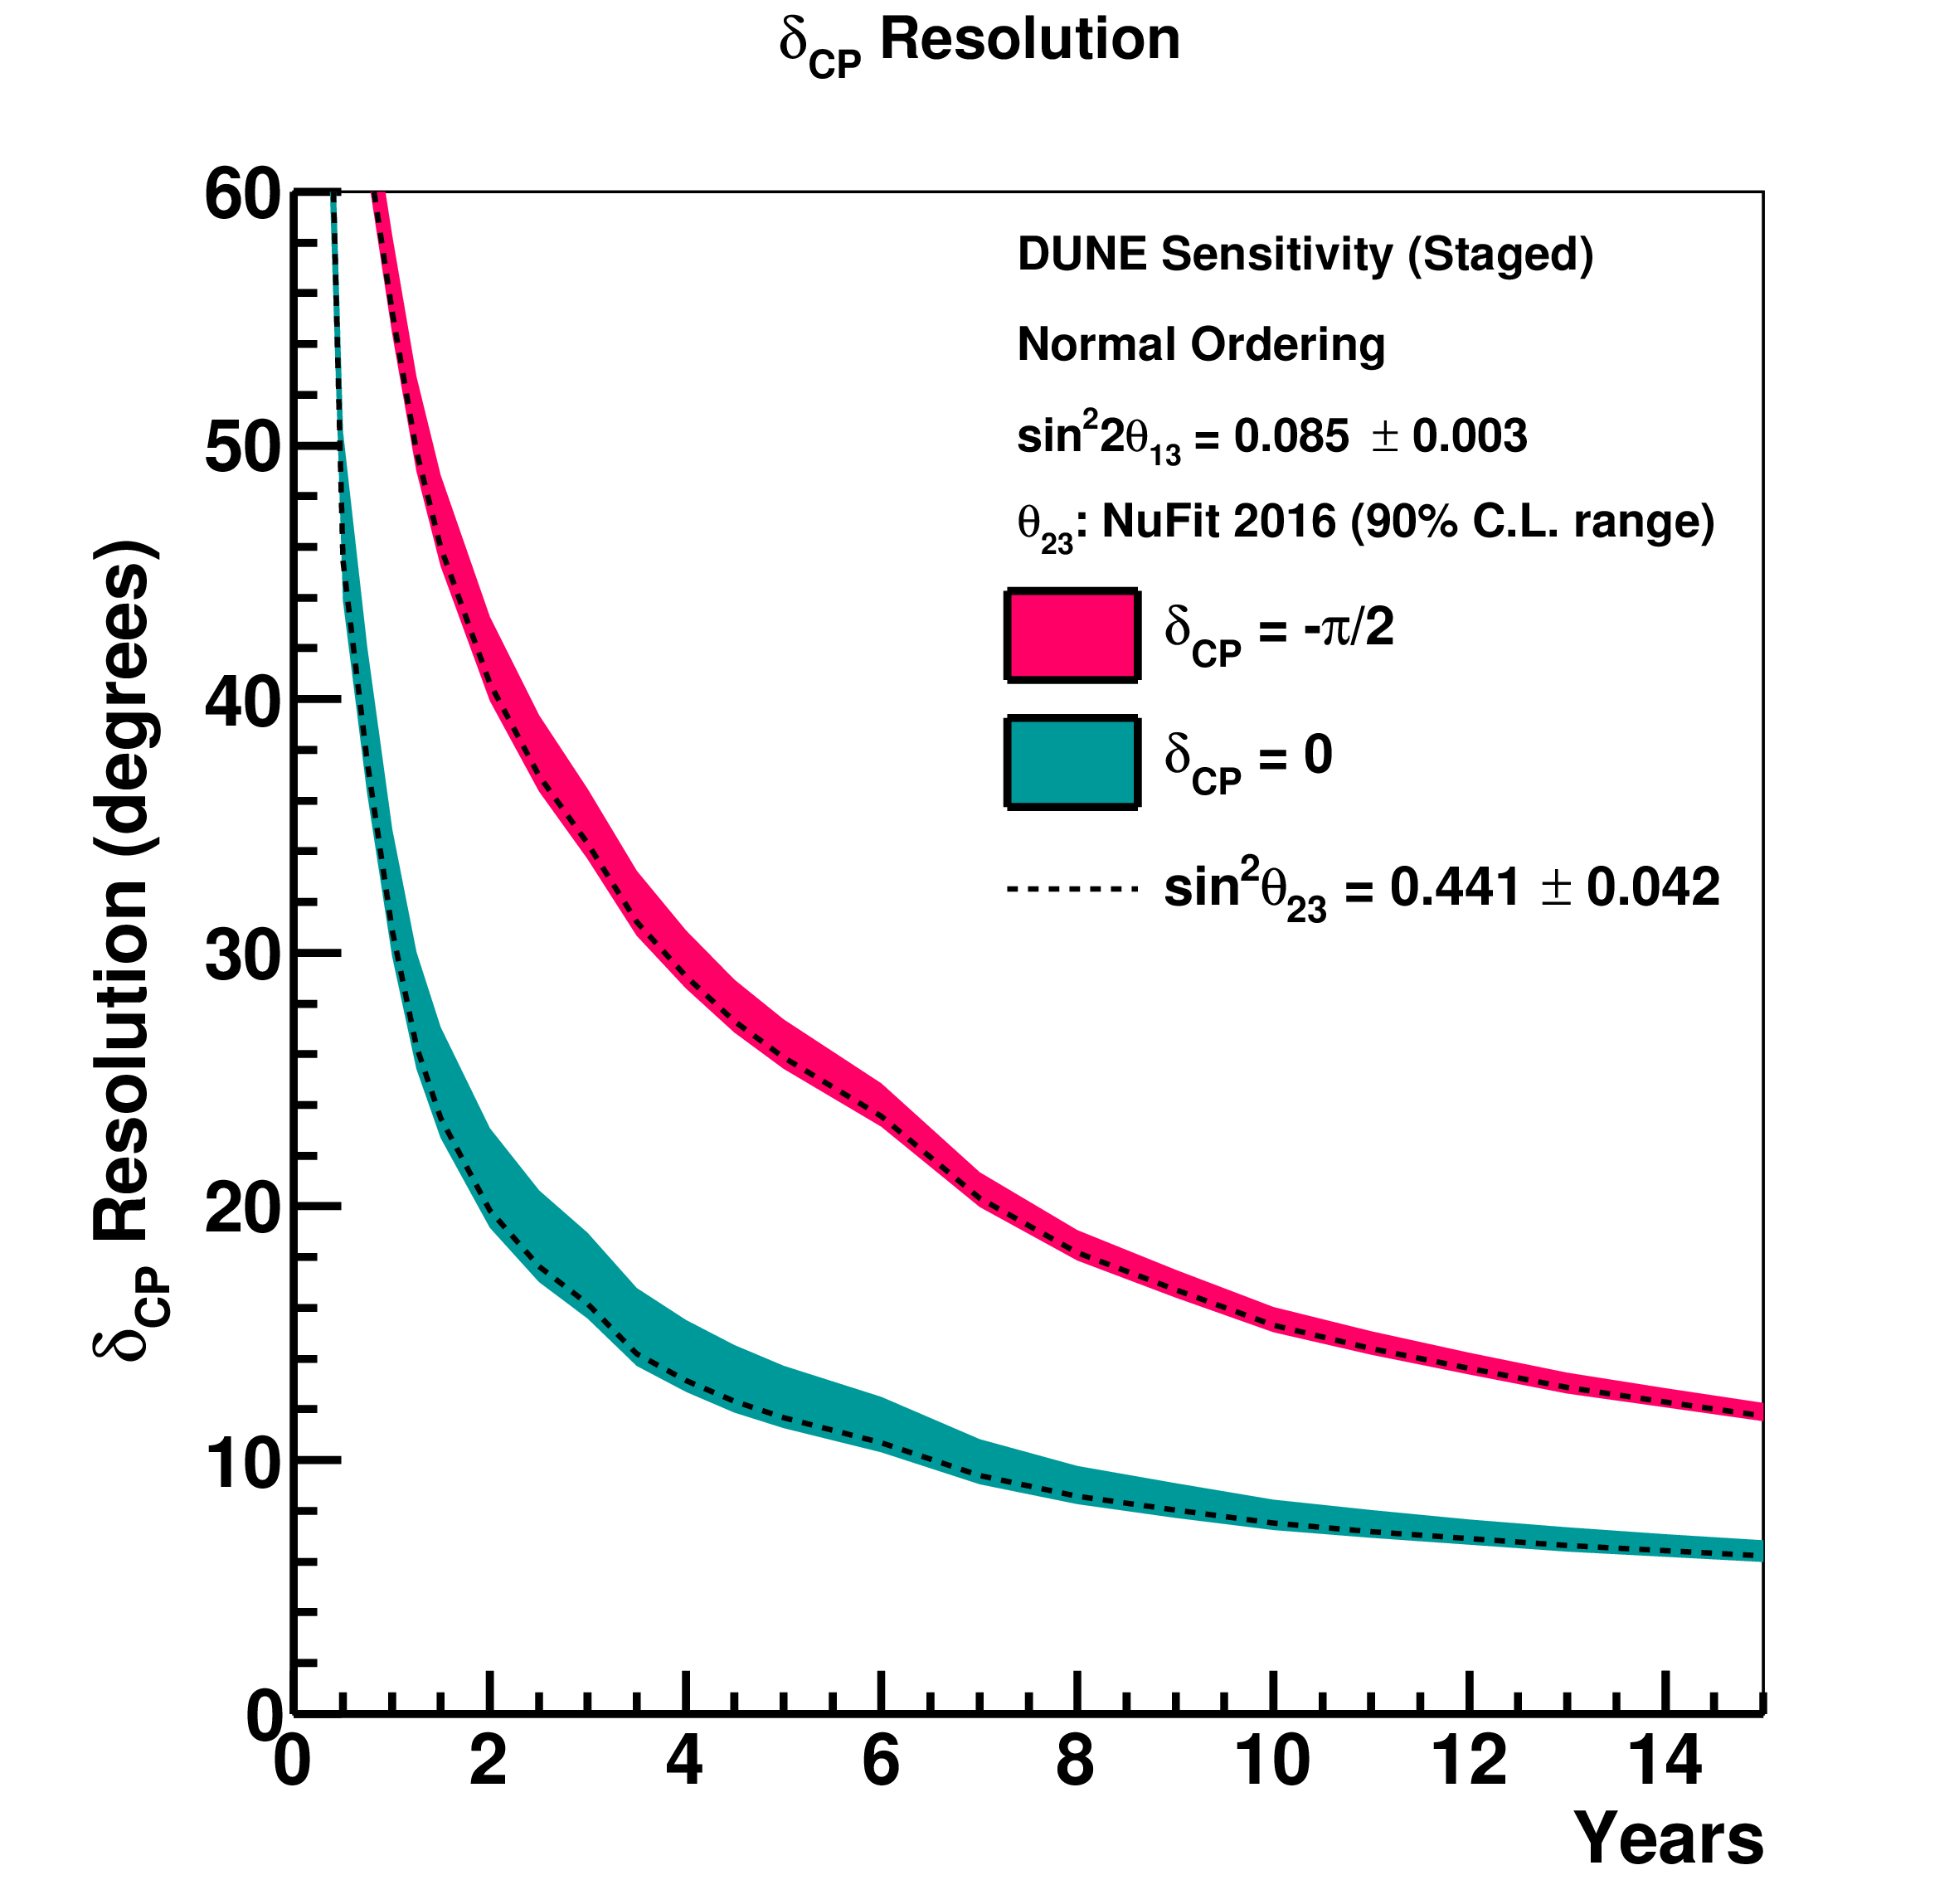
\includegraphics[width=0.49\textwidth]{resdcp_exp_staging_th23band_2017.png}
\label{fig:execsummaryCP}
\end{dunefigure}
%
Figure~\ref{fig:execsummaryCP} shows, as a function of time, the
expected sensitivity to CP violation expressed as the minimum significance
with which CP violation can be determined for 75\% and 50\% of
\deltacp values as well as the sensitivity when the true value of \deltacp=-$\pi$/2.
Also shown is the 1$\sigma$ resolution for \deltacp as a
function of time for $\delta_{\rm CP}=0$ (no CP violation) and
$\delta_{\rm CP}=90^\circ$ (maximal CP violation). In both figures the staging scenario
described above was assumed.  The exposure required to measure
$\delta_{\rm CP} = 0 $ with a precision better than $10^\circ$ is \SI{250}~\ktMWyr{} or about five years of operation. A full-scope LBNF/DUNE operating with 
multi-megawatt 
beam power can eventually achieve a precision 
comparable to the current precision on the CP phase in the
CKM matrix in the quark sector (5\%).

Table~\ref{tab:execosctable} summarizes the exposures needed to
achieve specific oscillation physics milestones, calculated 
for the current best-fit values of the known neutrino mixing parameters. 
For example, to reach $3\sigma$ sensitivity 
for 75\% of the range of \deltacp, a
DUNE exposure of \SI{775}~\ktMWyr{} or 12 years is needed. 
Changes in the assumed true value of
$\theta_{23}$ impact CP-violation and MH sensitivities and can either reduce or increase the 
discovery potential for CP violation, as seen in Fig.~\ref{fig:execsummaryCP}. To reach this level of sensitivity 
a highly capable near neutrino detector is required to control systematic uncertainties at a level lower than
the statistical uncertainties in the far detector. No experiment can provide coverage at 100\% of
\deltacp values, since CP-violating effects vanish as \mdeltacp to 0
or $\pi$.
 %
\begin{dunetable}[Required exposures to reach oscillation physics
  milestones]{lcc}{execosctable}{The exposure in mass (kt) $\times$ proton beam power
    (MW) $\times$ time (years) and calendar years assuming the staging plan described in this chapter needed to reach certain oscillation physics
    milestones. The numbers are for normal hierarchy using the NuFit 2016 best fit values of the known oscillation parameters.  }
Physics milestone & Exposure  & Exposure \\ \rowtitlestyle
  & (\ktMWyr{}) & (years) \\ \toprowrule 
  $1^\circ$ $\theta_{23}$ resolution ($\theta_{23} = 42^\circ$) & 29  &  1\\ \colhline
  CPV at $3\sigma$ ($\delta_{\rm CP} = -\pi/2$)  & 77 &  2\\ \colhline
  MH at  $5\sigma$ (worst point) & 209 & 5 \\ \colhline
  $10^\circ$ resolution ($\delta_{\rm CP} = 0$) & 252 & 5 \\ \colhline
  CPV at $5\sigma$ ($\delta_{\rm CP} = -\pi/2$)  & 253 & 5 \\ \colhline
  CPV at $5\sigma$ 50\% of \deltacp & 483 & 8 \\ \colhline
  CPV at $3\sigma$ 75\% of \deltacp & 775 & 12\\  \colhline
  Reactor $\theta_{13}$ resolution & 857 & 13 \\   
 ($\sin^2 2 \theta_{13} = 0.084 \pm 0.003$) &  &  \\  
\end{dunetable}
  
In long-baseline experiments with \numu beams, the
magnitude of \numu disappearance and \nue appearance signals is
proportional to \sinstt{23} and \sinst{13},

respectively, in the standard three-flavor mixing scenario.  Current
\numu disappearance data are consistent with close to maximal
mixing, $\theta_{23} = 45^\circ$.  To obtain the best sensitivity to
both the magnitude of its deviation from $45^\circ$ as well the 
$\theta_{23}$ octant, a combined analysis of the two channels
is needed~\cite{Huber:2010dx}.  A DUNE detector with sufficient exposure will be able to
resolve the $\theta_{23}$ octant at the $3\sigma$ level or better for
$\theta_{23}$ values less than $43^\circ$ or greater than $48^\circ$.
The full LBNF/DUNE scope will allow $\theta_{23}$ to be measured with a precision of
$1^\circ$ or less, even for values within a few degrees of
$45^\circ$. 

 DUNE has great prospects to discover CP violation or, in the absence of the
effect, set stringent limits on the allowed values of \deltacp. 
DUNE will also determine the neutrino mass hierarchy with better
than a $5\sigma$~C.L. and provide precision measurements
of the mixing angles $\theta_{23}$ and $\theta_{13}$.


%%%%%%%%%%%%%%%%%%%%%%%%%%%%%%%%%%%%%%%%%%%%%%%%%%%%%%%%%%%%%%%%%%%%%%%%%%%%%%%%%%
\section{Nucleon Decay and the GeV Scale Non-Accelerator Physics Program}

\subsection{Nucleon Decay}

Unification of three fundamental forces in the Universe, strong, electromagnetic and weak interactions, is largely seen as the next step in the development of particle physics model. Grand Unified Theories (GUTs), aiming at extending the Standard Model of particle physics to include a unified force at very high energies  (above $10^{15}$ GeV), predict a number of observable effects at low energies, such as nucleon decay (NDK) \cite{Pati1973,Georgi1974,Dimopoulos1982,Langacker1981,deBoer1994,Nath2007}. Several experiments have been searching for signatures of NDK with the best limits for most decay modes set by the Super-Kamiokande experiment \cite{Nishino2012} that features the largest sensitive mass to date. 

DUNE, as the largest LArTPC, will be searching for different NDK modes, having an advantage over Super-Kamiokande for observing nucleon decays into charged kaons that are below the Cherenkov threshold in water Cherenkov detectors. These modes are favored by the SUSY models and the tests of these models are within reach of multi-kiloton LArTPCs such as DUNE. One of the most promising modes of the proton decay search with DUNE $p\to K^+ \bar{\nu}$, expected to have a lifetime of the order of $>10^{33}$ years in SUSY models, can be tagged in LArTPC if a single kaon within a proper energy/momentum range can be reconstructed with its primary vertex to be within the fiducial volume. Background events initiated by cosmic-ray muons can be rejected by requiring no activity close to the edges of the TPCs and a single kaon identification within the energy range of interest. Atmospheric neutrino-induced background with a positive kaon production can either have an associated strange baryon (for reactions with $\Delta S = 0$) whose decay can be reconstructed, or a lepton (for reactions with $\Delta S = 1$) with reconstructed track or shower. 

Monte Carlo studies of this mode of proton decay and atmospheric neutrino background carried out within LArSoft framework with full event reconstruction, revealed that the main challenge in identifying proton decay candidates, is in mis-reconstruction of protons as positive kaons. This happens when a CC neutrino interaction produces a muon and a recoiling proton and the primary vertex for neutrino interaction is mis-labelled as a secondary vertex where the kaon decays. These mis-reconstructed events are primarily caused by the fact that final state interactions (FSI) in proton decay shift the spectrum of kaons towards low energies making difficult the energy and $dE/dx$ reconstruction, and kaon/proton separation. The work is ongoing, including neural networks, to improve background rejection for this mode of proton decay and to understand the uncertainty associated with the intra-nuclear cascade model (FSI). 

Currently best limit on this mode of proton decay has been set by Super-Kamiokande \cite{Abe2014}: $\tau/B > 5.9\times10^{33}$ years (90\% C.L.), obtained from a 260 kt$\cdot$year exposure~\cite{kearns_isoups}\footnote{The lifetime shown here is divided by the branching fraction for this decay mode, $\tau/B$, and
 as such is a \emph{partial lifetime}.}. The DUNE FD with more than 40 kt fiducial mass for these searches is expected to extend the sensitivity to $>10^{34}$ years. 

SUSY GUT models also favor other NDK modes involving positive or neutral kaons in the final state, for instance, $n\to K^+ e^-$. The cosmic-ray muon background for this decay mode is negligible whereas neutrino induced background is limited to CC reactions with $\Delta S = 1$ and mis-reconstructed events. 
We expect that the ProtoDUNE data with charged particle beams at CERN will provide important sample of events to train and improve on reconstruction algorithms. 

The DUNE FD will be sensitive to other NDK modes, such as $p\to \pi^0 e^+$ but in many cases the sensitivity will not exceed that of Super-Kamiokande.

The baryon number non-conservation can also be manifested by neutron-antineutron oscillations leading to the antineutron annihilation with a neutron or a proton. This annihilation event will have a distinct signature of a vertex with several emitted hadrons. The ability to re-construct these hadrons correctly and measure their energies is key to the identification of the signal event. The main background for these $n\bar n$ annihilation events is caused by atmospheric neutrinos. Most commonly mis-classified events are neutral current deep inelastic scattering events without a lepton in the final state. As above, final state interactions make picture more complicated and are probably the major component of the systematic uncertainty for the sensitivity studies.
Initial signal vs background discrimination studies have been performed using convolutional neural networks resulting in an equivalent sensitivity  of $n\rightarrow \bar n$ oscillation lifetime of $1.6 \times 10^9$~s at 90\% confidence level, a factor of 5 improvement on the current limit from Super-Kamiokande.
More information about particle identification and energy measurements will be provided by the ProtoDUNE experiment with charged particle beams. 

High efficiency of detecting NDK and $n\rightarrow \bar n$ enables a rich program of searches for baryon number non-conservation in the DUNE LArTPC detector.

\vspace{1cm}

List of references for this subsection.
\vspace{0.5cm}

J. C. Pati and A. Salam, Is Baryon Number Conserved?, Phys. Rev.vLett., vol. 31, pp. 661-
664, 1973.

H. Georgi and S. Glashow, Unity of All Elementary Particle Forces, Phys. Rev. Lett., vol. 32,
pp. 438-441, 1974.

S. Dimopoulos, S. Raby, and F. Wilczek, Proton Decay in Supersymmetric Models,
Phys. Lett., vol. B112, p. 133, 1982.

P. Langacker, Grand Unified Theories and Proton Decay, Phys. Rept., vol. 72, p. 185, 1981.

W. de Boer, Grand unified theories and supersymmetry in particle physics and cosmology,
Prog. Part. Nucl. Phys., vol. 33, pp. 201-302, 1994.

P. Nath and P. Fileviez Perez, Proton stability in grand unified theories, in strings and in
branes, Phys. Rept., vol. 441, pp. 191-317, 2007.

H. Nishino et al. (Super-Kamiokande Collaboration), Search for Nucleon Decay into Charged Anti-lepton plus Meson in Super-
Kamiokande I and II, Phys. Rev., vol. D85, p. 112001, 2012.

K. Abe et al. (Super-Kamiokande Collaboration), Search for proton decay via $p\to K^+ \bar{\nu}$ using 260 kiloton$\cdot$year data of Super-Kamiokande, Phys. Rev. D, 90 (2014) no.7, 072005. 


\subsection{Atmospheric neutrinos}

Atmospheric neutrinos are a unique tool to study neutrino oscillations: the oscillated flux contains all flavors of neutrinos and antineutrinos, is very sensitive to matter effects and to both $\Delta m^2$ parameters, and covers a wide range of $L/E$. In principle, all oscillation parameters could be measured, with high
complementarity to measurements performed with a neutrino beam. In addition, atmospheric neutrinos are available all the time, in particular before the beam becomes operational. The DUNE far detector, with its large mass and the overburden to protect it from atmospheric muon background, is an ideal tool for these studies.

The sensitivity to oscillation parameters has been evaluated with a dedicated, but simplified, simulation, reconstruction and analysis chain. The fluxes of each neutrino species at the far detector location were computed taking into account the oscillations. Interactions in the LAr medium were simulated with the GENIE
event generator. Detection thresholds and energy resolutions based on full simulations were applied to the outgoing particles, to take into account detector effects. Events were classified as Fully Contained (FC) or Partially Contained (PC) by placing the vertex at a random position inside the detector and tracking the lepton until its edges. The number of events expected for each flavor and category is summarized in Table \ref{table:atmnu-rates}.

Table \ref{table:atmnu-rates} summarizes event rates in the DUNE FD from atmospheric neutrinos.

\begin{table}[htp]
\caption{Atmospheric neutrino event rates per year in 40 kt fiducial mass of the DUNE FD.}
\begin{center}
\begin{tabular}{|c|c|}

\hline
Fully contained atmospheric $e$-like & $1.6\times10^{3}$ \\ \hline
Fully contained atmospheric $\mu$-like & $2.4\times10^{3}$ \\ \hline
Partly contained atmospheric $\mu$-like & $7.9\times10^{2}$ \\
\hline

\end{tabular}
\end{center}
\label{table:atmnu-rates}
\end{table}%

When neutrinos travel through the Earth, the MSW resonance influences electron neutrinos in the few-GeV energy range. More precisely, the resonance occurs for $\nu_e$ in the case of normal mass hierarchy (NH, $\Delta m^2 > 0$), and for $\bar \nu_e$ in the case of inverted mass hierarchy (IH, $\Delta m^2 < 0$). 
The mass hierarchy (MH) sensitivity can thus be greatly enhanced if neutrino and antineutrino events can be separated. The DUNE detector will not be magnetized; however, its high-resolution imaging offers possibilities for tagging features of events that provide statistical discrimination between neutrinos
and antineutrinos. Two tags can be used to discriminate $\bar \nu$  and $\nu$ events: a proton tag (a signature of neutrino interaction) and a positive muon decay tag (a signature of antineutrino interaction since only 25\% of negative muons will decay).

Unlike for beam measurements, the sensitivity to MH with atmospheric neutrinos is nearly independent of the CP-violating phase. The sensitivity comes
from both electron neutrino appearance as well as muon neutrino disappearance, and is strongly dependent on the true value of $\theta_{23}$. Despite the much smaller mass, DUNE would have comparable sensitivity to Hyper-Kamiokande atmospheric neutrino analyses due to better event reconstruction.
In the two-flavour approximation, neutrino oscillation probabilities depend on $\sin^2(2\theta)$, which is invariant when changing $\theta$ to $\pi/2 - \theta$. In this case, the octant degeneracy remains for $\theta_{23}$ in the leading order terms of the full three-flavor oscillation probability, making it impossible to determine whether $\theta_{23} < \pi/4$ or $\theta_{23} > \pi/4$. Accessing full three-flavor oscillation with atmospheric neutrinos may help to solve the ambiguity.

These analyses will provide a complementary approach to beam neutrinos. Atmospheric neutrinos can help to lift degeneracies that can be present in beam analyses, for instance, through the fact that the MH sensitivity is essentially independent of $\delta_{CP}$. Atmospheric neutrino data will be acquired even in the absence of the beam, and will provide a useful sample for the development of reconstruction software and analysis methodologies. Atmospheric neutrinos provide a window into a range of new physics scenarios, and can place limits on CPT violation \cite{Kostelecky2004}, non-standard interactions, mass-varying neutrinos \cite{Abe2008}, sterile neutrinos \cite{Abe2015}, and Lorentz invariance violation \cite{Kostelecky2012}.

Full Monte Carlo studies of the atmospheric neutrino effects in the detector are in progress.

\vspace{1cm}

List of references for this subsection.
\vspace{0.5cm}

V. A. Kostelecky and M. Mewes, Lorentz and CPT violation in neutrinos, Phys. Rev.,
vol. D69, p. 016005, 2004.

K. Abe et al., Search for Matter-Dependent Atmospheric Neutrino Oscillations in Super-Kamiokande, Phys. Rev., vol. D77, p. 052001, 2008.

K. Abe et al., Limits on sterile neutrino mixing using atmospheric neutrinos in Super-Kamiokande, Phys. Rev., vol. D91, p. 052019, 2015.

A. Kostelecky and M. Mewes, Neutrinos with Lorentz-violating operators of arbitrary dimension,
Phys. Rev., vol. D85, p. 096005, 2012.


%%%%%%%%%%%%%%%%%%%%%%%%%%%%%%%%%%%%%%%%%%%%%%%%%%%%%%%%%%%%%%%%%%%%%%%%%%%%%%%%%%
%\section{Supernova Neutrino Bursts and Physics with Low-Energy Neutrinos}
\section{Supernova-Neutrino Physics and Astrophysics}

The neutrinos from a core-collapse supernova are emitted in a burst of
a few tens of seconds duration, with about half the signal emitted in the first
second. The neutrino energies are mostly in the range 5--50 MeV, and the
luminosity is divided roughly equally between the three known neutrino
flavors.  Current water and scintillator detectors are sensitive primarily to
electron antineutrinos ($\bar{\nu}_e$), with detection through the inverse-beta decay
process on free protons\footnote{This refers to neutrino interactions with the nucleus of a
hydrogen atom in H$_2$O in water detectors or in hydrocarbon chains in 
liquid scintillator detectors.},
 which dominates the interaction rate in these detectors.  Liquid argon has a unique sensitivity to
the electron-neutrino ($\nu_e$) component of the flux, via the absorption
interaction on $^{40}$Ar,
\begin{eqnarray*}
\nu_e +{}^{40}{\rm Ar} & \rightarrow & e^-+{}^{40}{\rm K^*}.
\end{eqnarray*} 
This interaction can in principle be tagged via the coincidence of the emitted
electron and the accompanying photon cascade from the $^{40}{\rm K^*}$
de-excitation.  About \num{3000} events would be expected in a \ktadj{40}
fiducial mass liquid argon detector for a supernova at a distance of
\SI{10}{\kilo\parsec}.  In the neutrino channel, the oscillation
features are in general more pronounced, since the $\nu_e$ spectrum is almost
always significantly different from the $\nu_\mu$ ($\nu_\tau$) spectrum 
in the initial core-collapse stages, to a larger degree than is the
case for the corresponding $\bar{\nu}_e$ spectrum.  
While $\nu_e$ absorption should represent $\sim$90\% of the signal, there are in addition other channels of interest, including $\bar{\nu}_e$ charged current, elastic scattering on electrons (which provides pointing information) and neutral-current
interactions which result in final-state deexcitation $\gamma$'s. 
Each channel has a distinctive signature in the detector, but in all cases events appear as small (tens of cm scale) tracks and blips.   Figure~\ref{fig:snb} shows an example of a simulated event.  Section~\ref{sec:sb} describes reconstruction and calibration challenges for these events.


Observation of the core-collapse neutrino burst in DUNE
will provide critical information on key
astrophysical phenomena~\cite{Mirizzi:2015eza}.  These include the neutronization burst, for which the initial sharp, bright flash
of $\nu_e$ from  $p+e^- \rightarrow n + \nu_e$
heralds the formation of a compact neutron star remnant.
The collapse of the proto-neutron star into a black hole would be signaled by a sharp cutoff in neutrino flux.
Shock wave effects, shock instability oscillations, turbulence effects, and transitions to quark stars could all produce observable features in the energy, flavor and time structure of the neutrino burst.
Furthermore, detection of the supernova burst 
neutrino signal in DUNE will give information on neutrino properties: see reference~\cite{Mirizzi:2015eza}.  Most notably, several features offer multiple signatures of mass ordering~\cite{Scholberg:2017czd}, likely the most robust being the level of suppression of the  neutronization burst: see Fig.~\ref{fig:snb}.  Because the neutronization burst is $\nu_e$-rich, this mass ordering signature is especially clean in DUNE.
``Collective effects'', due to self-induced transitions driven by \textit{neutrino-neutrino interactions} in the dense matter of the supernova, result in a rich phenomenology with multiple observables primarily at later times.  


\begin{dunefigure}[]{snb}{Left: Event display of a 30-MeV neutrino event simulated using MARLEY. Right: Expected event rates as a function of time for the electron-capture supernova model in~\cite{Huedepohl:2009wh} for 40 kt of argon during early stages of the event--- the neutronization burst and early accretion phases, for which self-induced effects are unlikely to be important.  Shown is the event rate for the unrealistic case of no flavor transitions (blue), the event rate including the effect of matter transitions for the normal (red)  and inverted (green) hierarchies.  Error bars are statistical, in unequal time bins.}
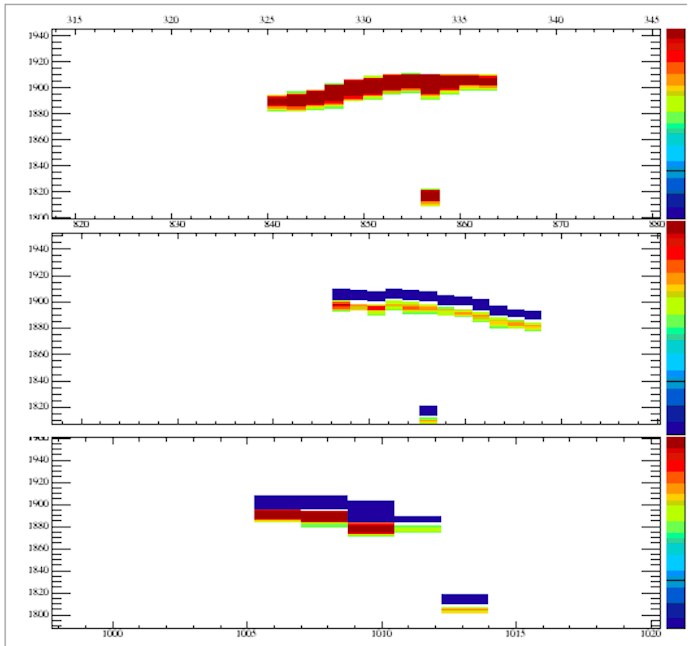
\includegraphics[width=0.29\textwidth]{snb-event-display.png}
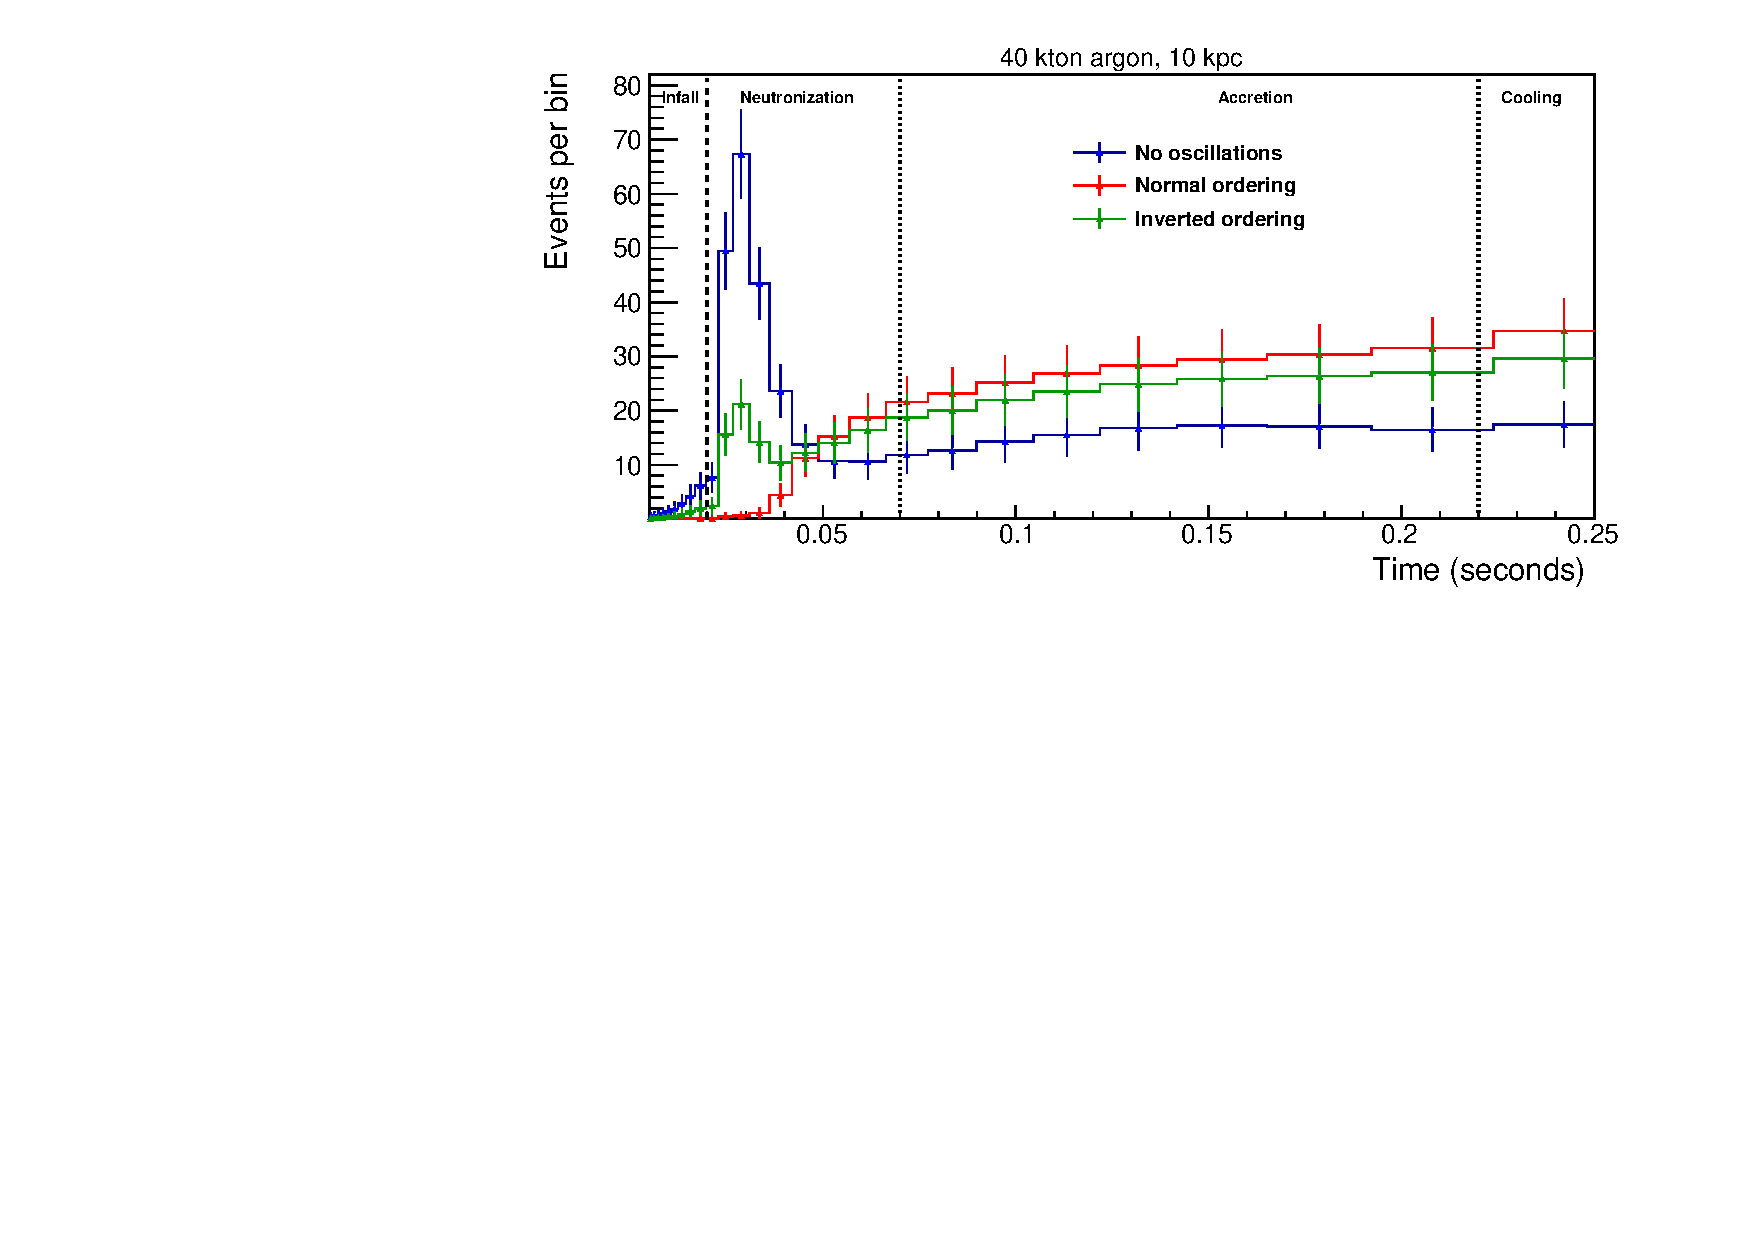
\includegraphics[width=0.6\textwidth]{early_time_argon.pdf}
\label{fig:snb}
\end{dunefigure}

Because no beam trigger is available for a supernova, efficient triggering and data collection is critical for supernova neutrino burst physics.   

We note that DUNE information will be highly complementary with neutrino burst information from other detectors, and furthermore multimessenger astronomy information (from gravitational waves and a broad range of electromagnetic wavelengths) will combine to provide a full picture of a core-collapse event.



%%%%%%%%%%%%%%%%%%%%%%%%%%%%%%%%%
\section{Precision Measurements with the DUNE Near Detector Complex}
\label{sec:exec-summ-nd-precision-physics}

The DUNE near detector
will provide precision measurements of
neutrino interactions that are essential
for controlling the systematic uncertainties in the long-baseline
oscillation physics program.  The near detector 
will include argon targets and will measure the absolute flux and energy-dependent
shape of all four neutrino species, \numu, \anumu, \nue and \anue,
to accurately predict for each species the
far/near flux ratio as a function of energy.  It will also measure the
four-momenta of secondary hadrons, such as charged and neutral mesons,
produced in the neutral- and charged-current interactions that
constitute the dominant backgrounds to the oscillation signals.

The near detector will also be the source of data for a rich program
of neutrino-interaction physics in its own right. For an integrated
beam intensity of \num{1e20} 
protons-on-target at \SI{120}{GeV}, the expected number of events per
ton is \num{170000} (\num{59000}) 
\numu (\anumu) charged-current and \num{60000} (\num{25000}) neutral-current interactions in the $\nu$ ($\overline\nu$) beam\footnote{With PIP-II, the integrated protons-on-target per year is
  expected to be around $1.1\times 10^{21}$ at \SI{120}\GeV. The mass
  of the Ar target in the Low-mass Tracker option for the DUNE ND is expected to be approximately
  100~kg.}. 
  These numbers correspond to \num{e5} neutrino interactions
on argon per year for the range of beam configurations and near detector
designs under consideration.  Measurement of fluxes, cross sections
and particle production over a large energy range of
\SIrange{0.5}{50}{\GeV} are the key elements of this program.  These
data will also help constrain backgrounds to proton-decay signals
from atmospheric neutrinos.  Furthermore, very large samples of events
will be amenable to precision reconstruction and analysis, and will be
exploited for sensitive studies of electroweak physics and nucleon
structure, as well as for searches for new physics in unexplored
regions, such as heavy sterile neutrinos, high-$\Delta m^2$
oscillations, and light Dark Matter particles. %, and so on.

%%%%%%%%%%%%%%%%%%%%%%%%%%%%%%%%%%%%%%%%%%%%%%%%%%%%%%%%%%%%%%%%%%%%
%\section{Auxiliary Physics Program}
%\label{sec:exec-summ-physics-aux}
\section{Opportunities in Beyond the Standard Model Physics}
%\section{Additional opportunities for Beyond Standard Model Physics}
\label{sec:exec-summ-physics-bsm}
The unique combination of the high-intensity LBNF neutrino beam with DUNE's near detector and massive LArTPC far detector modules at a 1300 km baseline enables a variety of probes of Beyond the Standard Model Physics, either novel or with unprecedented sensitivity. This section describes a selection of such topics, and briefly summarizes how DUNE can make leading contributions in this arena.

\subsection{New Particle Searches}
{\bf Search for Low-mass Dark Matter.}
Various cosmological and astrophysical observations strongly support the existence of Dark Matter (DM) representing $\approx$27$\%$ of the mass-energy of the universe, but its nature and potential non-gravitational interactions with regular matter remain undetermined. 
The lack of evidence for Weakly Interacting Massive Particles (WIMP) at direct detection and the LHC experiments resulted in a reconsideration of the WIMP paradigm. For instance, if DM has a mass which is much lighter than the electroweak scale (e.g., below the GeV level), it motivates theories for DM candidates that interact with ordinary matter through a new "vector portal" mediator.
High flux neutrino beam experiments, such as DUNE, have been shown to provide coverage of DM+$mediator$ parameter space which cannot be covered by either direct detection or collider experiments[1-4]. Upon striking the target, the proton beam can produce dark photons either directly through $pp(pn)\rightarrow V$ or indirectly through the production of a $\pi^{0}$  or a $\eta^{0}$ meson, which then promptly decays into SM photons of which one of them couples to a dark photon. If $m_V>2m_{DM}$, the dark photons will quickly decay into a pair of DM particles, which then travel along with the neutrinos to the DUNE near detector, where they can be detected through neutral-current-like interactions either with electrons or nucleons in the detector material.
%Since the signature of DM events looks just like those of the neutrinos, the neutrino beam provides the major source of background for the DM signal. 
The neutrino-induced backgrounds can be suppressed using the arrival time difference of the DM in the near detector with respect to neutrinos and the angle of the scattered electrons, taking advantage of the fine angular resolution DUNE can provide.  These enable DUNE's search for LDM be competitive and complementary to other experiments.\\

{\bf Search for Boosted Dark Matter}
Using its large far detector, DUNE will be able to search for boosted dark matter (BDM), where DM is produced relativistically.
A representative model is composed of heavy and light DM components and the lighter one can be produced from the annihilation of the heavier one in a region where the heavy DM components are clumpy enough, e.g., Galactic Center, Sun (depending on the model construction), or dwarf spheroidal galaxies.
Due to the large mass difference between the two DM components, the lighter one is produced relativistically.
The incoming energy of the lighter DM component can be high enough above the expected energy thresholds of DUNE in a wide range of parameter space. 
The excellent resolution in identifying particles and their position and propagation angles provides DUNE with unique abilities in detecting the BDM signal, in particular when the boosted light DM scatters on protons, or inelastic scattering happens as expected in the more generalized set up of inelastic BDM ({\it i}BDM).
A first attempt at observing the {\it i}BDM signal with ProtoDUNE prior to running DUNE is proposed in Ref.~\cite{sample} and the same analysis strategy can be used in the corresponding study at DUNE.
%The conventional DM search via its non-relativistic scattering is not accessible because the typical energy deposit resulting from the ordinary DM scattering is much below than the detector recoil threshold energy. In contrast, typical energy deposits in association with a relativistic scattering of the boosted DM readily surpass such a threshold. Hence, DUNE far detector with large fiducial volume and excellent detector technology will be an ideal detector to search for boosted DM.

{\bf Heavy Neutral Leptons.}
The high intensity of the LBNF neutrino beam and the production of charm mesons in the beam enable DUNE to search for a wide variety of lightweight long-lived, exotic particles, by looking for topologies of rare event interactions and decays in the fiducial volume of the DUNE Near Detector. These particles include weakly-interacting Heavy Neutral Leptons - right-handed partners of the active neutrinos, vector, scalar, or axion portals to the Hidden Sector, and light super-symmetric particles.  
%There are other experiments around the world that  such a measurement can complement with its particular geometry of 660 m of earth protecting the ND. 
%We particularly focus on decay-in-flight of sub-GeV particles that are also candidates for dark matter and a good explanation of leptogenesis in the case of CP violoation indications. The main guiding models we use is the dark photon and heavy neutral lepton decays. 
Assuming these heavy neutral leptons are the lighter particles of their hidden sector, they will only decay in SM particles in the form of pairs like $e^+ e^-$  , $\mu^+\mu^-$ , $q\,\bar{q}$ . 
The parameter space explored by the DUNE near detector extends into the cosmologically relevant region complementary to the LCH heavy-mass dark-matter searches through missing energy and mono-jets. 
%The SHiP experiment being constructed at CERN will be contemporary to the DUNE measurements at the time of its operation [ref-HNL].

%{ref-HNL, SHiP sets a new course in intensity-frontier exploration, CERN Courier, http://cerncourier.com/cws/article/cern/63982}


\subsection{Searches for Deviations from the PMNS Neutrino Mixing Paradigm}
{\bf Non-Standard Neutrino Interactions.}
Non-standard neutrino interactions, affecting neutrino propagation through the Earth, can significantly modify the data to be collected by DUNE as long as the new physics parameters are large enough~\cite{Masud:2015xva}. Leveraging its very long baseline and wide-band beam, DUNE is uniquely sensitive to  these probes. If the DUNE data are consistent with standard oscillations for three massive neutrinos, interaction effects of order 0.1 $G_F$ can be ruled out at DUNE~\cite{deGouvea:2015ndi,Coloma:2015kiu}. We notice that DUNE might improve current constraints on $\epsilon_{\tau e}$ and $\epsilon_{\mu e}$ by a factor 2-5~\cite{Farzan:2017xzy}.

{\bf Non-Unitarity.} 
A generic characteristic of most models explaining the neutrino mass
pattern is the presence of heavy neutrino states, additional to the
three light states of the Standard Model of particle
physics~\cite{Minkowski:1977sc,Mohapatra:1979ia,Yanagida:1979as,GellMann:1980vs}. This imply a deviation from unitary of the $3\times3$ PMNS matrix, which can be particularly sizable the lower the mass of the extra states~\cite{Mohapatra:1986bd,Akhmedov:1995vm,Akhmedov:1995ip,Malinsky:2005bi}.
For values of the unitarity deviations of order $10^{-2}$, this would decrease the expected reach of DUNE to the standard parameters, although stronger bounds existing from charged leptons would be able to restore its expected performance~\cite{Blennow:2016jkn,Escrihuela:2016ube}.

{\bf Violations of Lorentz or CPT Symmetry.}
CPT symmetry, the combination of Charge Conjugation, Parity and Time reversal, is a cornerstone of our model building strategy and therefore the repercussions of its potential violation will severely threaten the standard model of particle physics. DUNE can improve the present limits on CPT violation by several orders of magnitude~\cite{Streater:1989vi,Barenboim:2002tz,Barenboim:2017ewj}, being a very important experiment to test one of the deepest results of quantum field theory.

{\bf Active-Sterile Neutrino Mixing.}
Experimental results in tension with the three-neutrino-flavor paradigm~\cite{LSNDSterile,MiniBooNESterile,GalliumSummary,ReactorSummary}, which may be interpreted as mixing between the known active neutrinos and one or more {\it sterile} states, have led to a rich and diverse program of searches for oscillations into sterile neutrinos.
DUNE is sensitive over a broad range of potential sterile neutrino mass splittings by looking for disappearance of CC and NC interactions over the long baseline separating the Near and Far detectors, as well as over the short baseline of the Near detector. Results from the MINOS and NOvA long-baseline accelerator experiments~\cite{MINOSSterile2016, NOvASterile2017} have demonstrated the validity of this approach. With a longer baseline, a more intense beam, and a high-resolution large-mass Far detector, DUNE provides a unique opportunity to improve significantly on the sensitivities of the existing probes, and greatly enhance the ability to map the extended parameter space if a sterile neutrino is discovered.

{\bf Large Extra-Dimensions.}
DUNE can search for or constrain the size of large extra-dimensions (LED) by looking for distortions of the oscillation pattern predicted by the three-flavor paradigm. These distortions arise through mixing between the right-handed neutrino Kaluza-Klein modes, which propagate in the compactified extra dimensions, and the active neutrinos, which exist only in the four-dimensional brane~\cite{LEDModel}. Searching for these distortions in, for instance, the $\nu_\mu$~CC disappearance spectrum should provide significantly enhanced sensitivity over existing results from the MINOS/MINOS+ experiment~\cite{MinosplusLED}.

{\bf Neutrino Trident Production.}
The intriguing possibility that neutrinos may be charged under new gauge symmetries beyond the Standard Model (SM) $SU(3)_c\times SU(2)_L\times U(1)_Y$, and interact with the corresponding new gauge bosons can be tested with unprecedented precision by DUNE through Near detector measurements of neutrino-induced di-lepton production in the Coulomb field of a heavy nucleus, also known as {\it neutrino trident} interactions~\cite{Altmannshofer:2014pba}. Although this process is extremely rare (SM rates are suppressed by a factor of $\sim 10^{-5}-10^{-7}$ with respect to CC interactions), the CHARM-II collaboration \cite{Geiregat:1990gz} and the CCFR collaboration \cite{Mishra:1991bv} both reported detection of several trident events ($\sim 40$ events at CCFR) and quoted cross-sections in good agreement with the SM predictions. With a predicted annual rate of over 100 di-muon neutrino trident interactions at the Near detector, DUNE will be able to measure deviations from the SM rates and test for the presence of new gauge symmetries.


%\fixme{2 pages, make case that DUNE is best/unique, high level}

%%%%%%%%%%%%%%%%%%%%%%%%%%%%%%%%%%%%%%%%%%%%%%%%%%%%%%%%%%%%%%%%%%%%%%%%%
\section{Summary}

In summary, the primary science goals of DUNE are drivers for the
advancement of particle physics. The questions being addressed are of wide-ranging consequence: the origin of flavor and the generation
structure of the fermions, the physical mechanism that provides the CP
violation needed to generate the baryon asymmetry of the universe, 
and the high-energy physics that would lead to the instability
of matter.  Achieving these goals requires a dedicated, ambitious and
long-term program.  No other proposed long-baseline neutrino
oscillation program with the scientific scope and sensitivity of DUNE
is as advanced in terms of engineering development and project
planning.  The staged implementation of
the far detector as four 10-kt modules will enable
exciting physics in the intermediate term, including a definitive mass
hierarchy determination and possibly a measurement of the CP phase, 
while providing the fastest route toward achieving the
full range of DUNE's science objectives.  Should DUNE find that the CP
phase is not zero or $\pi$, it will have found strong indications
($>3\sigma$) of leptonic CP violation.

The DUNE experiment is a world-leading international physics
experiment, bringing together the 
international neutrino community as well as leading experts in nucleon decay
and particle astrophysics to explore key questions at the forefront of
particle physics and astrophysics. The highly capable beam and
detectors will enable a large suite of new physics measurements with
potentially groundbreaking discoveries.



